
Given,
\begin{align}
\tag{24.1}
    F_{X}(x)=\begin{cases} 
            0  &  x<0\\
            x &  0 \le x <1/2\\
            \frac{\brak{1+x}}{2} &  1/2 \le x <1\\
            1  &  x\ge 1
            \end{cases} \label{ma2018-24:a}
\end{align}
\begin{align}
\tag{24.2}
    \pr{X=1/2}=\pr{X\leq 1/2}-\pr{X<1/2} 
\end{align}
\begin{align}
\tag{24.3}
    \implies \pr{X=1/2}=F_{X}\brak{\frac{1}{2}}-F_{X}\brak{\frac{1}{2}^-} \label{ma2018-24:b}
\end{align}
 Using \eqref{ma2018-24:a} in \eqref{ma2018-24:b},
\begin{align}
\tag{24.4}
    \implies \pr{X=1/2}=\frac{\brak{1+1/2}}{2}-\brak{1/2}\\
\tag{24.5}
    \implies \pr{X=1/2}=\brak{3/4}-\brak{1/2}
\end{align}
\begin{align}
\tag{24.5}
    \therefore \pr{X=1/2}=1/4
\end{align}
The cdf plot of random variable X is as shown in Fig. \ref{ma2018-24:cdf_plot}\\
\begin{figure}[t!]
    \centering
    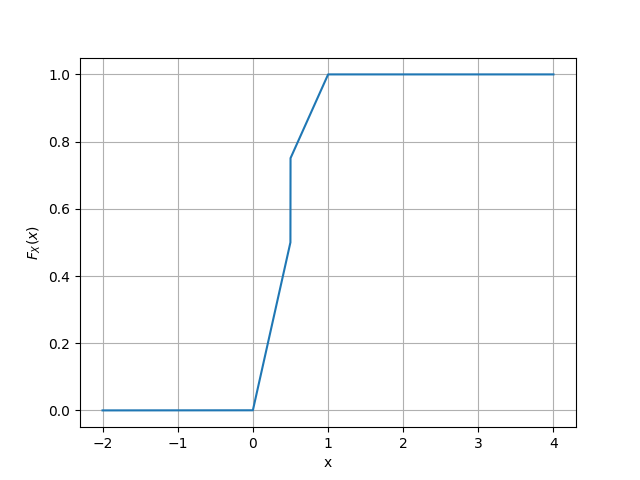
\includegraphics[width=\columnwidth]{solutions/adv/ma/2018/24/cdf_plot.png}
    \caption{cdf plot of random variable X}
    \label{ma2018-24:cdf_plot}
\end{figure}
